%%%%%%%%%%%%%%%%%%%%%%%%%%%%%%%%%%%%%%%%%%%%%%%%%%%%%%%%%%%%%%%%%%%%%%%%%%%%%%%
% Chapter 'Absorption - Water - Libr/CH3CH(OH)COONa ratio 2/1'
%%%%%%%%%%%%%%%%%%%%%%%%%%%%%%%%%%%%%%%%%%%%%%%%%%%%%%%%%%%%%%%%%%%%%%%%%%%%%%%
\subsection{Libr/ch3ch(oh)coona ratio 2/1}
%
%%%%%%%%%%%%%%%%%%%%%%%%%%%%%%%%%%%%%%%%%%%%%%%%%%%%%%%%%%%%%%%%%%%%%%%%%%%%%%%
%%%%%%%%%%%%%%%%%%%%%%%%%%%%%%%%%%%%%%%%%%%%%%%%%%%%%%%%%%%%%%%%%%%%%%%%%%%%%%%
\subsubsection{Antoine - ID 1}
%
\begin{tabular}[l]{|lp{11.5cm}|}
\hline
\addlinespace

\textbf{Sorbent:} & Libr/CH3CH(OH)COONa \\
\textbf{Subtype:} & ratio 2/1 \\
\textbf{Refrigerant:} & Water \\
\textbf{Equation:} & Antoine \\
\textbf{ID:} & 1 \\
\textbf{Reference:} & Lucas, Antonio de; Donate, Marina; Rodríguez, Juan F. (2006): Vapour pressures, densities, and viscosities of the (water+lithium bromide+potassium acetate) system and (water+lithium bromide+sodium lactate) system. In: The Journal of Chemical Thermodynamics 38 (2), S. 123–129. DOI: 10.1016/j.jct.2005.04.007. \\
\textbf{Comment:} & None \\

\addlinespace
\hline
\end{tabular}
\newline

\textbf{Equation and parameters:}
\newline
%
Pressure $p$ in $\si{\pascal}$ is calculated depending on concentration $X$ in $\si{\kilogram\per\kilogram}$ and  temperature $T$ in $\si{\kelvin}$ by:
%
\begin{equation*}
\nicefrac{p}{d} = 10 ^ { \sum_{i=0}^{4} \left( A_i + \frac{1000 B_i}{T - c} \right) \left( 100 X \right) ^{i}}
\end{equation*}
%
The parameters of the equation are:
%
\begin{longtable}[l]{lll|lll}
\toprule
\addlinespace
\textbf{Par.} & \textbf{Unit} & \textbf{Value} &	\textbf{Par.} & \textbf{Unit} & \textbf{Value} \\
\addlinespace
\midrule
\endhead

\bottomrule
\endfoot
\bottomrule
\endlastfoot
\addlinespace

$c$ & $\si{\kelvin}$ & 4.315000000e+01 & $d$ & $\si{\pascal}$ & 1.000000000e+03 \\
$A_0$ & - & 6.770000000e+00 & $B_0$ & $\si{\kelvin}$ & -1.640000000e+00 \\
$A_1$ & - & 5.110000000e-03 & $B_1$ & $\si{\kelvin}$ & 5.260000000e-04 \\
$A_2$ & - & -2.200000000e-04 & $B_2$ & $\si{\kelvin}$ & -5.790000000e-07 \\
$A_3$ & - & 0.000000000e+00 & $B_3$ & $\si{\kelvin}$ & 0.000000000e+00 \\
$A_4$ & - & 0.000000000e+00 & $B_4$ & $\si{\kelvin}$ & 0.000000000e+00 \\

\addlinespace\end{longtable}

\textbf{Validity:}
\newline
Equation is approximately valid for $298.15 \si{\kelvin} \leq T \leq 333.15 \si{\kelvin}$.
\newline

\textbf{Visualization:}
%
\begin{figure}[!htp]
{\noindent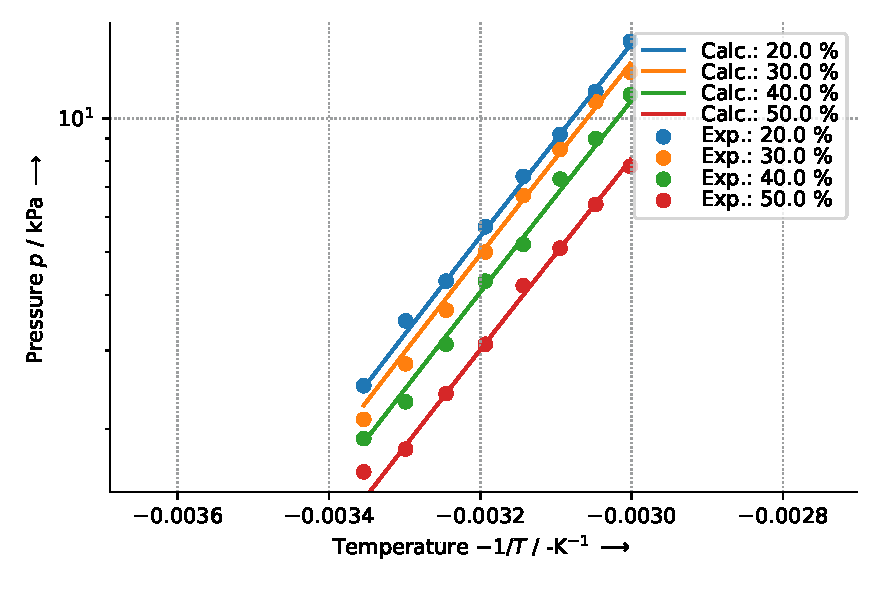
\includegraphics[height=10cm, keepaspectratio]{figs/abs/abs_Water_Libr_CH3CH(OH)COONa_ratio_2_1_Antoine_1.pdf}}
\end{figure}
%

To generate the figure, the following refrigerant functions were selected:
\begin{itemize}
\item Vapor pressure: VaporPressure\_EoS1 - ID 1
\item Saturated liquid density: SaturatedLiquidDensity\_EoS1 - ID 1
\end{itemize}

The uncertainity of the experimental data is:
\begin{itemize}
\item Data source $\,\to\,$ Data was taken from table
\item Pressure, absolute, in $\si{\pascal}$ $\,\to\,$ 100
\item Temperature, absolute, in $\si{\kelvin}$ $\,\to\,$ 0.01
\item Concentration / Molar fraction, absolute, in $\si{\kilogram\per\kilogram}$ / $\si{\mole\per\mole}$ $\,\to\,$ 1.00E-07
\end{itemize}

The mean absolute percentage error (MAPE) between the experimental and calculated data results in 3.31\%.
\FloatBarrier
\newpage
%%%%%%%%%%%%%%%%%%%%%%%%%%%%%%%%%%%%%%%%%%%%%%%%%%%%%%%%%%%%%%%%%%%%%%%%%%%%%%%
